\hypertarget{empiricalModels}{
}

%\begin{itemize}
%	\item{Lambertian}
%	\item{Phong, Blinn-Phong}
%	\item{Ward}
%	\item{Lafortune}
%\end{itemize}

\noindent For the texture synthesis of the materials, various local reflection \footnote[1]{Another set of reflection models are global illumination models. These are beyond the scope of this thesis.} models can be used. This chapter will outline the empirical models used in the process of texture synthesis. These models capture reflectance behaviour using mathematical models without using any basic laws of physics. Such models are widely used for their simplicity and because they can be controlled by setting only a small set of parameters to obtain desired results.

\section{Lambertian reflectance}\label{Lambertian}
	One of the most used empirical models is Lambertian reflectance. In computer graphics, this model is mainly used to model diffuse reflectance. Surfaces with such properties appear equally bright from all viewing angles because the light is reflected with equal intensity in all directions. The brightness of the surface is only dependent of the angle $\theta$ between the surface normal $\vec{\mathbf{n}}$ and the light source direction $\vec{\mathbf{l}}$ as shown in figure X. We can look at a diffuse surface on microscopic level to understand how this works. 

If we look at \ref{fig:BEAM}, we can see how an incoming light beam projects a differential area $dA$ on the surface. If the surface normal and the light direction are parallel and in the same direction as shown in figure \ref{fig:BEAM}, the energy the area receives and reflects is proportional to $dA$. If the beam is projected on the surface such that it covers a larger area as shown in \ref{fig:BEAM}, the amount of energy reflected from area $dA$ is proportional to $\cos \theta$. The amount of energy reflected per unit area is less on surface 2 compared to surface 1 since the beam covers a larger area. This observation of radiance behaviour is also known as Lambert's Cosine Law. In general, for Lambertian reflectance, the amount of light observed by the viewer is indepenendent of the viewing angle, and is only dependent on the angle of the incidence of the light source. The full equation is given by:

		\begin{eqnarray*}
			I = I_pk_d\cos\theta
		\end{eqnarray*}

Here, $I$ is the reflected amount of light, $I_p$ is the intensity of the light source, $k_d$ is the \tit{diffuse reflection coefficient} which varies between 0 and 1 and is material dependent. The cosine term is defined between $0^0$ and $90^0$. This means that the surface is treated as self-occluding; angles outside this range will result in negative values for the cosine term and are treated as a $max({0,\cos\theta})$, resulting in zero intensity falling on the surface. If both $\vec{\mathbf{n}}$ and $\vec{\mathbf{l}}$ are normalized, we can write the equation as:

		\begin{eqnarray*}
			I = I_pk_d(\vec{\mathbf{n}} \cdot \vec{\mathbf{l}})
		\end{eqnarray*}

This model is used effectively for the synthesis of diffuse surfaces and in interactive software since the reflection term doesn't need to be recomputed whenever the view changes. However, most materials are deviating from Lambertian for angles of view or incidence greater than $60^0$ \cite{DigitalModeling}. Another shortcoming of Lambertian reflectance is that it does not include the observation of speculars on materials. For these reasons the model is insufficient to synthesize materials with a more glossy nature since they will need the speculars to be present. 


\begin{figure}[H]
	\begin{center}
		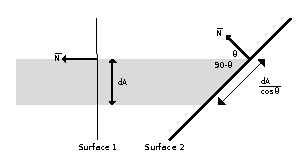
\epsfig{file=images/beam_example.eps, width=0.5\linewidth}
	\end{center}
	\caption{Beam shown in gray, projecting an area on surfaces. The projected area on surface 1 equals $dA$, and on surface 2 equals $\frac{dA}{\cos\theta}$. \tit{Image adapted from Computer Graphics, Principles and Practice \cite{ComputerGraphics}}}
	\label{fig:BEAM}
\end{figure}




	\section{Phong Reflectance}\label{Phong}
		With the Lambertian assumption of light reflecting equally into all direction, we can expect poor quality synthesis when we're dealing with more glossy/specular surfaces such as metallic, stone and plastic materials. As Bui-Tuong Phong wrote in his article, if the goal in shading a computer-synthesized image is to simulate a real physical object, then the shading model should in some way imitate real physical shading situations \cite{Phong}. Phong reflectance is a popular model, based on the empirical observation of how shiny surfaces can have small specular highlights, and how these observed speculars are related to the view direction of the observer.
The general idea of Phong reflection is shown in figure \ref{fig:SPECULAR1}. Here we have an incident angle $\theta_i$ and an equal reflection angle $\theta_r$. The incident light is reflected into the direction of $\vec{\mathbf{R}}$

\begin{figure}[H]
	\begin{center}
		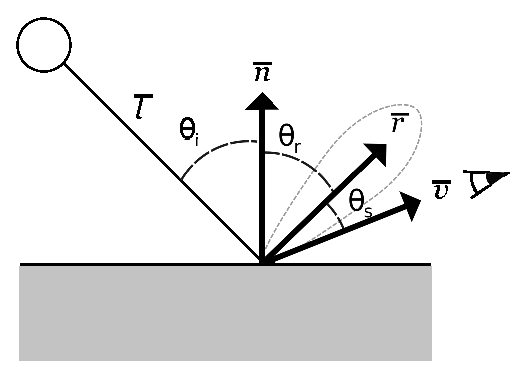
\epsfig{file=images/specular_reflection.eps, width=0.4\linewidth}
	\end{center}
	\caption{Specular reflection. $\theta_i$ is the angle of the incoming light, and is equal to the reflected angle $\theta_r$. $\alpha$ is the angle between the view direction and the reflected light.}
	\label{fig:SPECULAR1}
\end{figure}

	\section{Blinn-Phong Reflectance}\label{BlinnPhong}

